\section{Реализация кросс-архитектурной миграции}

В рамках исследований был реализован механизм кросс-архитектурной миграции процесса Linux с архитектуры x86 на архитектуру ARM. Мы совместили подход проекта CRIU, и получили состояние процесса исключительно средствами пространства пользователя, с эмулятором qemu, для получения кросс-архитектурной трансляции. При реализации миграции процесса мы ограничились только двумя ресурсами: памятью процесса и состоянием процессора.

Процедура миграции процесса состоит из двух частей создания образа и восстановления процесса из образа (checkpoint/restart). Для создания образа процесса сначала необходимо остановить процесс. Для этого в ОС Linux используется системный вызов ptrace. Системный вызов ptrace используется для отладки, он позволяет останавливать и возобновлять процесс, читать и изменять память процесса, читать и изменять содержимое регистров, перехватывать различные события, например, системные вызовы или сигналы~\cite{PTRACEP1,PTRACEP2}. Далее необходимо сохранить адресное пространство процесса и состояние регистров процессора.

Восстановление процесса осуществляется в эмуляторе qemu. Для восстановления процесса необходимо восстановить копию адресного пространства процесса в памяти qemu, затем восстановить состояние процессора.

\begin{figure}[h]
  \center{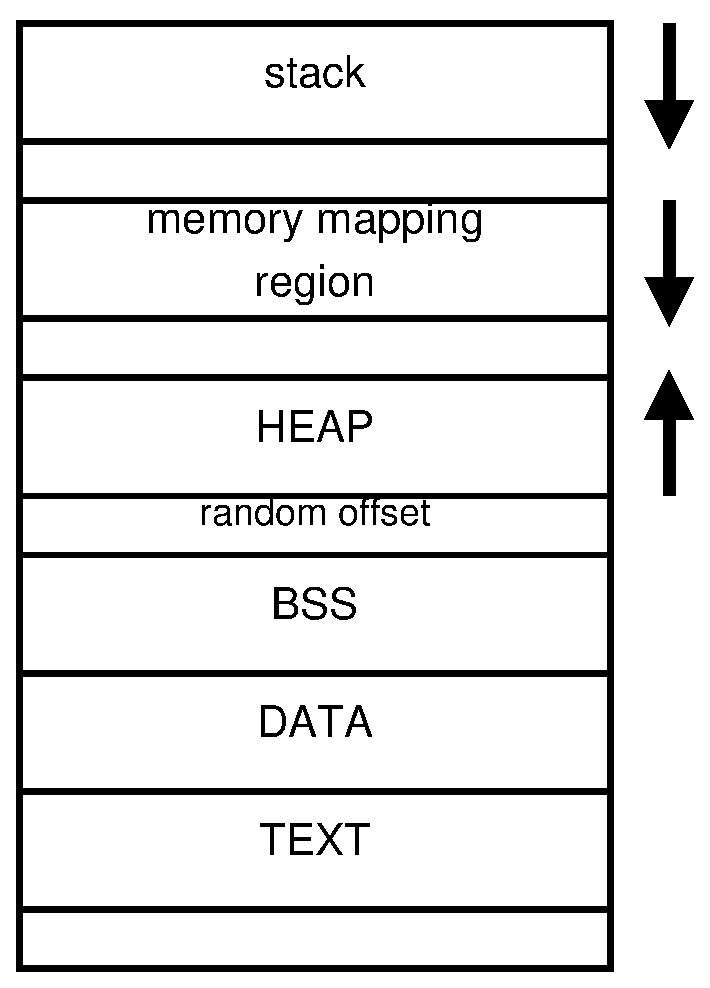
\includegraphics[width=0.8\linewidth]{memmap}}
  \caption{Адресное пространство процесса Linux}
  \label{img:memmap}
\end{figure}

Типичное адресное пространство процесса Linux изображено на рис.~\ref{img:memmap}. В самых верхних адресах адресного пространства располагается стек процесса, стек растет вниз. Ниже стека располагается memory mapping region, в этот регион памяти, обычно, загружаются динамические библиотеки, так же в этом регионе памяти выделяется память с помощью системного вызова mmap, этот регион растет вниз. Далее идет куча процесса, эта память используется для динамического выделения памяти, например, с помощью malloc или оператора new языка C++. Куча процесса растет вверх, верхняя граница определяется с помощью системных вызовов brk и sbrk. Нижние адреса занимает код и данные, память для которых была выделена на этапе компиляции. Таким образом адресное пространство процесса используется неравномерно, т. е. незанятые регионы памяти располагаются в середине адресного пространства процесса.

Чтобы получить содержимое памяти процесса в реализации используется файловая система proc. Список занятых регионов адресного пространства процесса доступен в файле /proc/<pid>/maps. Каждый регион памяти описывается диапазоном адресов, правами доступа (на чтение, запись и исполнение), а так же описанием (например, [HEAP], [STACK], /usr/lib/libc.so), т. е. чем занят данный регион памяти. Формат описания регионов памяти поддерживается постоянным, для обеспечения обратной совместимости.

Для считывания непосредственно памяти процесса используется файл /proc/<pid>/mem. Смещения в этом файле соответствуют адресам в адресном пространстве процесса, т. е. чтобы получить всю память процесса необходимо прочитать данные из этого файла согласно описаниям регионов памяти из файла /proc/<pid>/maps.

Восстановление адресного пространства процесса в эмуляторе qemu осуществляется с помощью системного вызова mmap. Память восстанавливается с сохранением относительных смещений регионов памяти, так как эмулятор не поддерживает сложных механизмов преобразования адресов в режиме эмуляции одного процесса.

Получение состояния регистров процессора осуществляется посредством команды PTRACE\_GETREGSET, системного вызова ptrace. В реализации мы ограничились только базовым набором регистров, т. е. регистры общего назначения, сегментные регистры, указатели стека и команд.

Восстановление состояния процессора в эмуляторе является тривиальной задачей, каждый поддерживаемый процессор в эмуляторе qemu описывается структурой языка C, а восстановление сводится к заполнению соответствующих полей структуры.
